%%%%%%%%%%%%%%%%%%%%%%%%%%%%%%%%%%%%%%%%%
% Beamer Presentation
% LaTeX Template
% Version 1.0 (10/11/12)
%
% This template has been downloaded from:
% http://www.LaTeXTemplates.com
%
% License:
% CC BY-NC-SA 3.0 (http://creativecommons.org/licenses/by-nc-sa/3.0/)
%
%%%%%%%%%%%%%%%%%%%%%%%%%%%%%%%%%%%%%%%%%

%----------------------------------------------------------------------------------------
%	PACKAGES AND THEMES
%----------------------------------------------------------------------------------------

\documentclass{beamer}

\mode<presentation> {

% The Beamer class comes with a number of default slide themes
% which change the colors and layouts of slides. Below this is a list
% of all the themes, uncomment each in turn to see what they look like.

%\usetheme{default}
%\usetheme{AnnArbor}
%\usetheme{Antibes}
%\usetheme{Bergen}
%\usetheme{Berkeley}
%\usetheme{Berlin}
%\usetheme{Boadilla}
%\usetheme{CambridgeUS}
%\usetheme{Copenhagen}
%\usetheme{Darmstadt}
%\usetheme{Dresden}
%\usetheme{Frankfurt}
%\usetheme{Goettingen}
%\usetheme{Hannover}
%\usetheme{Ilmenau}
%\usetheme{JuanLesPins}
%\usetheme{Luebeck}
\usetheme{Madrid}
%\usetheme{Malmoe}
%\usetheme{Marburg}
%\usetheme{Montpellier}
%\usetheme{PaloAlto}
%\usetheme{Pittsburgh}
%\usetheme{Rochester}
%\usetheme{Singapore}
%\usetheme{Szeged}
%\usetheme{Warsaw}

% As well as themes, the Beamer class has a number of color themes
% for any slide theme. Uncomment each of these in turn to see how it
% changes the colors of your current slide theme.

%\usecolortheme{albatross}
%\usecolortheme{beaver}
%\usecolortheme{beetle}
%\usecolortheme{crane}
%\usecolortheme{dolphin}
%\usecolortheme{dove}
%\usecolortheme{fly}
%\usecolortheme{lily}
%\usecolortheme{orchid}
%\usecolortheme{rose}
%\usecolortheme{seagull}
%\usecolortheme{seahorse}
%\usecolortheme{whale}
%\usecolortheme{wolverine}

%\setbeamertemplate{footline} % To remove the footer line in all slides uncomment this line
%\setbeamertemplate{footline}[page number] % To replace the footer line in all slides with a simple slide count uncomment this line

%\setbeamertemplate{navigation symbols}{} % To remove the navigation symbols from the bottom of all slides uncomment this line
}

\usepackage{graphicx} % Allows including images
\usepackage{booktabs} % Allows the use of \toprule, \midrule and \bottomrule in tables
\usepackage{amsmath}

%----------------------------------------------------------------------------------------
%	TITLE PAGE
%----------------------------------------------------------------------------------------

\title[Model Evaluation]{Model Evaluation} % The short title appears at the bottom of every slide, the full title is only on the title page

\author{David Bethge \& Fabio Ferreira} % Your name
\institute[] % Your institution as it will appear on the bottom of every slide, may be shorthand to save space
{
DHBW Karlsruhe \\ % Your institution for the title page
\medskip
\textit{} % Your email address
}
\date{\today} % Date, can be changed to a custom date

\begin{document}

\begin{frame}
\titlepage % Print the title page as the first slide
\end{frame}

\begin{frame}
\frametitle{Overview} % Table of contents slide, comment this block out to remove it
\tableofcontents % Throughout your presentation, if you choose to use \section{} and \subsection{} commands, these will automatically be printed on this slide as an overview of your presentation
\end{frame}


%----------------------------------------------------------------------------------------
%	PRESENTATION SLIDES
%----------------------------------------------------------------------------------------

%------------------------------------------------
\begin{frame}
\frametitle{recommended literature}
\begin{figure}
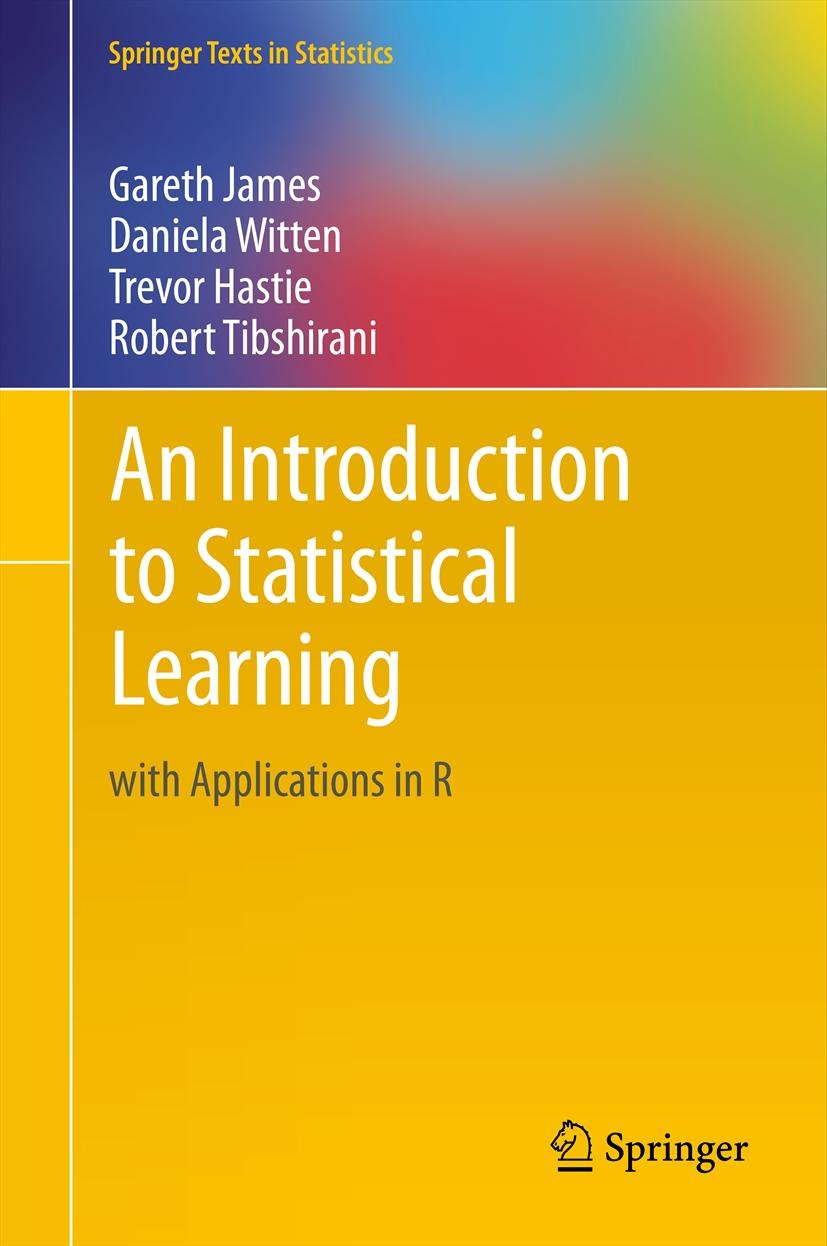
\includegraphics[width =.4\linewidth]{figures/03/Literature2.jpg}
\end{figure}

\end{frame}


\begin{frame}
\frametitle{Why do we need evaluation?}
Once you have defined your problem and prepared your data you need to apply machine learning algorithms to the data in order to solve your problem. You can spend a lot of time choosing, running and tuning algorithms. You want to make sure you are using your time effectively to get closer to your goal.
\newline
\newline
In this post you will step through a process to rapidly test algorithms and discover whether or not there is structure in your problem for the algorithms to learn and which algorithms are the most effective.
\end{frame}

\section{error term composition}
\begin{frame}
\frametitle{Example (1) }
First we need to understand more about the errors that can incur when doing machine learning:
\newline
Left plot: income vs. years of education for 30 individuals
suggests that one might be able to predict income using years of education

\begin{figure}
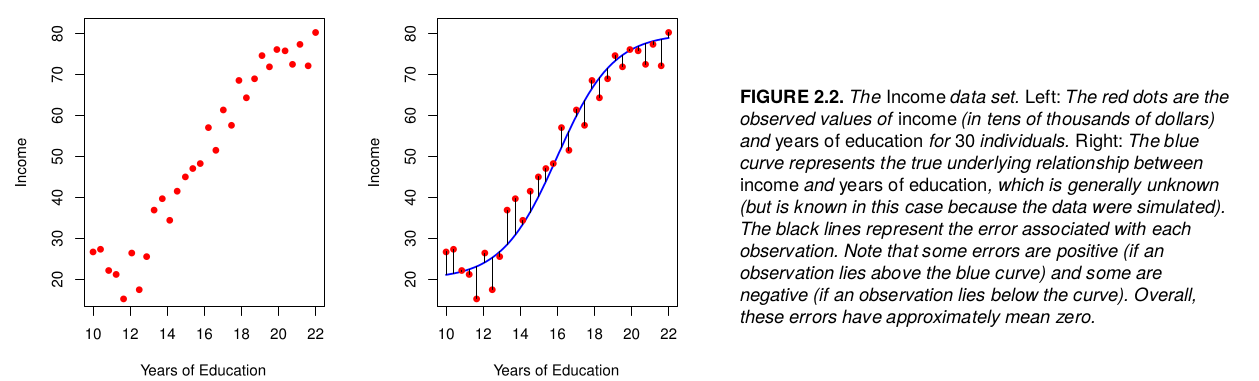
\includegraphics[width = 1\linewidth]{figures/03/figure_2_2.png}
%link statistical learning book
\end{figure}
\end{frame}

\begin{frame}
\frametitle{Example (2)}
\begin{itemize}
\item income is a simulated data set $f$ is known (blue curve, right plot)
\item vertical lines are random deviations (error terms) from $f$
\item Observations lie above and below the blue curve (overall with approx. mean zero) Deviations are denoted $\epsilon$
\item in general, the function $f$ may involve more than one input variable(e.g. expertise, job requirements,...) .
\end{itemize} 
\end{frame}


\begin{frame}
\frametitle{Example (3) }
Plot of income as a function of years of education \textbf{AND} seniority.
\newline
Since the error term averages to zero, we predict $y$ as $y = f(X)$
\begin{figure}
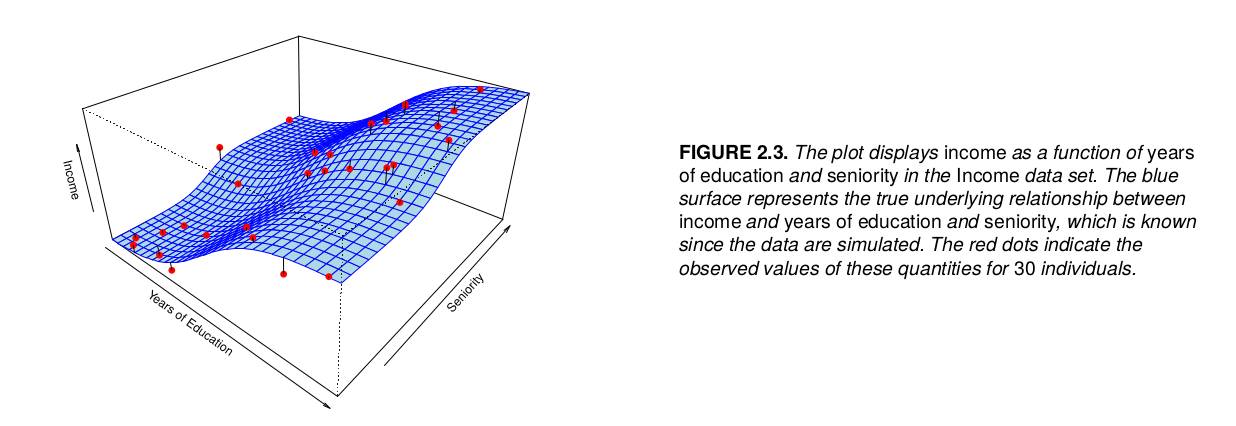
\includegraphics[width = 1\linewidth]{figures/03/figure_2_3.png}
%link statistical learning book
\end{figure}

\begin{itemize}
\item $\hat{f}(X)$ is our estimate for $f$
\item $\hat{y}$ is the resulting prediction for $y$
\end{itemize}
\end{frame}


\begin{frame}
\frametitle{reducible vs. irreducible error}
Accuracy of the prediction $\hat{y}$ for $y$ depends on two error types
\begin{itemize}
\item \textbf{Reducible error }
		\begin{itemize}
		\item in practice, $\hat{f}$ will not be a perfect estimate for $f$
        \item This inaccuracy will introduce some error
        \item Error is reducible because we can potentially improve the accuracy of $f$ by
using the most appropriate model to estimate $f$
		\end{itemize}
        \item \textbf{Irreducible error}
        \begin{itemize}
        \item Assuming a perfect estimate of $f$
        \item Prediction would still have some error because $y$ is also a function of $\epsilon$
        \item $\epsilon$‪ can by definition not be predicted using X
        \end{itemize}
        \item Therefore $\epsilon$ ‪also affects the accuracy of our predictions
        \item This irreducible error cannot be reduced – no matter how well try
\end{itemize}
\end{frame}

\begin{frame}
\frametitle{What can the error term tell us?}
\begin{itemize}
\item $\epsilon$ may contain unmeasured variables
\item These variables might be useful in predicting $Y$
\item However, we cannot use them for prediction as we don’t measure them
\item $\epsilon$ may also contain unmeasurable variation, e.g.
the risk of an adverse reaction might vary for a given patient on a given
day, depending on manufacturing variation in the drug itself or the patient’s
general feeling of well-being on that day
\item Finding systematics in $\epsilon$ can be exploited to adjust models (and gain
insights)
\end{itemize}
\end{frame}


\begin{frame}
\frametitle{Expected value and variance}
\begin{itemize}
\item Consider a given estimate $f$ and a set of predictors X
\item Assume $\hat{f}$ and X are fixed
\end{itemize}
\begin{equation*}
\mathbb{E}[y-\hat{y}]^2 = \mathbb{E}[f(X) + \epsilon -\hat{f}(X)]^2  = \underbrace{\mathbb{E}[f(X)-\hat{f}(X) ]^2 }_{reducible}  +\underbrace{Var(\epsilon)}_{irreducible} 
\end{equation*}
\end{frame}

\section{flexibility and fitting}
\begin{frame}
\frametitle{parametric vs. non-parametric methods}
Most statistical learning methods can be characterized as either
\newline
\textbf{ parametric or non-parametric}
\newline
We will now focus on parametric models:
Parametric Methods involve a two-step model-based approach
\begin{itemize}
\item \textbf{Shaping}: making an assumption about the functional shape of $f$
e.g. that $f$ is linear in X: $f(X) = \beta_0 + \beta_0X_1 + \beta_2X_2 + ... + \beta_p X_p$
\item Only p + 1 coefficients must be estimated
\item \textbf{Fitting}: stimating the parameters of the chosen model
\newline
In case of the linear model we need to estimate the parameters $\beta_0 ,‪\beta_1 ,‪...‪,‪\beta_p$ such that $Y \sim \beta_0 + \beta_0X_1 + \beta_2X_2 + ... + \beta_p X_p$  (e.g. via OLS)
\end{itemize}
 
\end{frame}

\begin{frame}
\frametitle{parametric models - pros \& cons}
Potential disadvantage of a parametric approach:
\begin{itemize}
\item The chosen model will usually not match the true unknown form of $f$
\item If the chosen model is too far from the true $f$, the estimate will be poor
\item This problem can be addressed by choosing flexible models that can fit many different possible functional forms for $f$
\item However: fitting a more flexible model in general requires estimating a
greater number of parameters
\newline
\item More complex models can lead to overfitting the data: 
A phenomenon known which essentially means that we follow the errors,
or noise, too closely
\end{itemize}
\end{frame}

\begin{frame}
\frametitle{Fitting Income Data with Linear
Regression}
 applying the parametric approach to the Income data
We fit a linear model of the form
\begin{equation*}
income \sim \beta_0 + \beta_1 education+ \beta_2 seniority
\end{equation*}
\begin{figure}
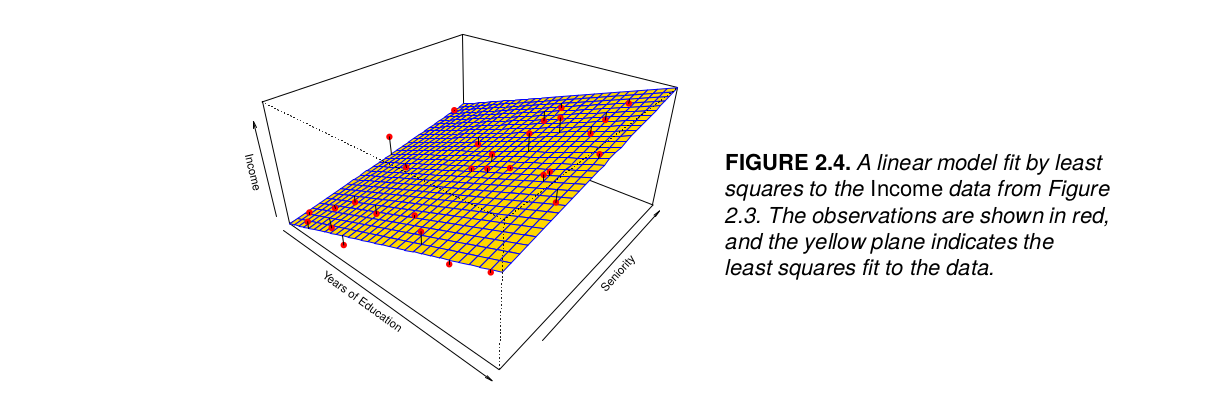
\includegraphics[width = 1.1\linewidth]{figures/03/figure_2_4.png}
%link statistical learning book
\end{figure}

\end{frame}


\begin{frame}
\frametitle{Fitting Income Data with Linear
Regression}
applying a non-parametric approach (splines)
\begin{itemize}
\item pre-specified model is imposed on $f$
\item A $\hat{f}$ is produced that is as close as possible to observed data
\item The fit (the surface) must be smooth (to a certain extent)
\item To fit a thin-plate spline, a level of smoothness must be chosen
\end{itemize} 
In this case, the non-parametric fit is a remarkably accurate estimate
\begin{figure}
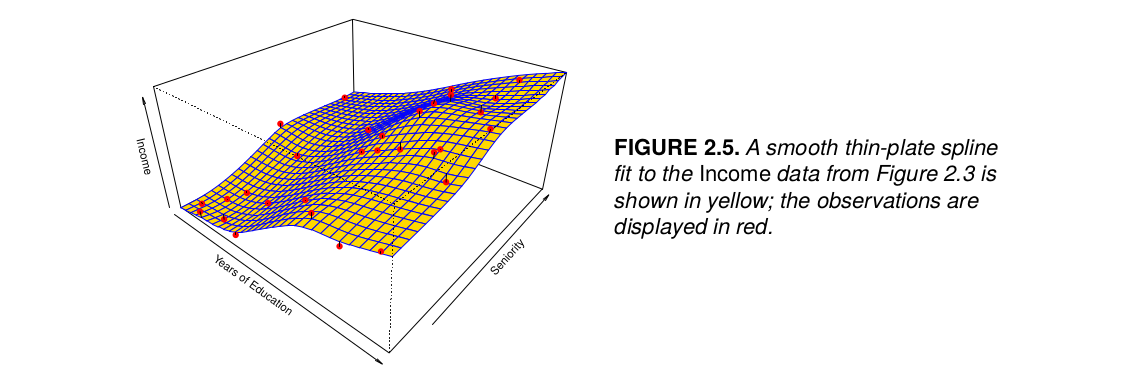
\includegraphics[width = 1.1\linewidth]{figures/03/figure_2_5.png}
%link statistical learning book
\end{figure}

\end{frame}

\begin{frame}
\frametitle{Whats the problem with flexibility?}
\textbf{Question}:
„Why‪ would ‪we‪ ever‪ choose‪ to‪ use‪ a ‪more ‪restrictive‪
prediction‪ model ‪instead ‪of ‪a‪ very ‪flexible‪ approach?“
\newline
\begin{itemize}
\item We might expect that it will be best to use the most flexible model 
\item Surprisingly, this is not the case!
\item Less flexible method often result in more accurate predictions
\item This phenomenon results from overfitting in highly flexible methods
\end{itemize}
\end{frame}


\section{test error}
\begin{frame}
\frametitle{Measuring the Quality of Fit: (Training) MSE}
\begin{itemize}
\item Evaluating the performance of a model / method on a given data set:
\item measuring how well its predictions match the observed data
\end{itemize}

\bigskip
\begin{itemize}
\item In a regression setting mean squared error (MSE) is commonly used
\item With $\hat{f}(x_i)$ as the prediction for the i-th observation of $y, y_i$:
\end{itemize}
\begin{equation*}
MSE = \frac{1}{n}\sum_{i=0}^n (y_i- \hat{f}(x_i))^2
\end{equation*}
\end{frame}

\begin{frame}
\frametitle{ Training vs. Test MSE}
\begin{itemize}
\item \textbf{Training MSE}: introduced MSE is computed using the training data that was used to fit the model
\item What‘s the accuracy when we apply our method to unseen test data? e.g., tomorrow‘s sales or next month’s cost of goods
\end{itemize}
\bigskip
Mathematically, we ...
\begin{itemize}
\item ... fit our method on training observations ${(x_1 , y_1 ), (x_2 , y_2 ), . . . , (x_n , y_n )}$
\item ... obtain estimate $\hat{f}$
\item ... compute $\hat{f}(x_1) , \hat{f}(x_2) , ... , \hat{f}(x_n) \rightarrow \hat{f}(x_0)$ 
\end{itemize}
However: we want to know whether $\hat{f}(x_0) \sim y_0$ for $(x_0 , y_0 )$ not used to train the method
\newline
Goal: Choosing the model with lowest test MSE (vs. training MSE)
\end{frame}


\begin{frame}
\frametitle{How to minimize Test MSE}
Simply selecting a statistical learning method that
minimizes the training MSE?
\begin{itemize}
\item There is a fundamental problem with this strategy:
\begin{itemize}
\item training set MSE can be quite small
\item test MSE is often much larger
\end{itemize} 
\item Where does this effect come from?
\item How are training and test MSE related?
\end{itemize}
\end{frame}


\begin{frame}
\frametitle{Training vs. Test MSE}

\begin{figure}
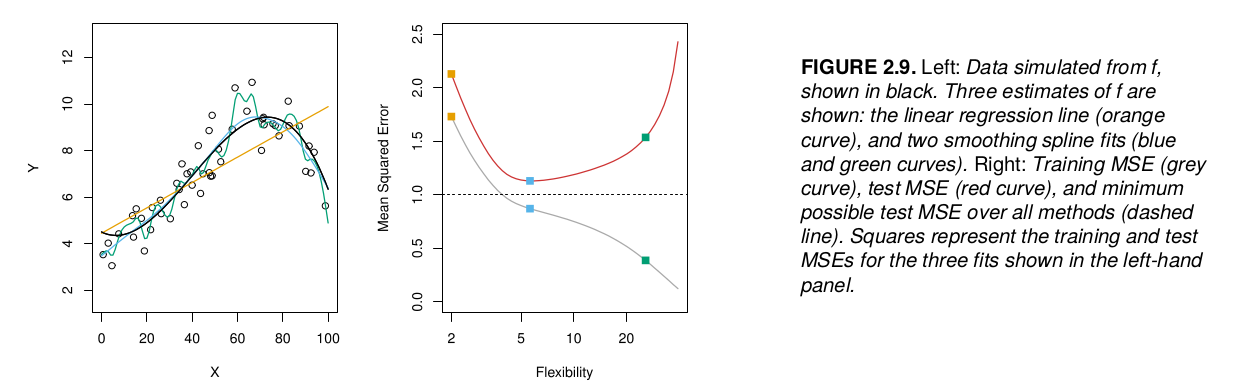
\includegraphics[width = 1\linewidth]{figures/03/figure_2_6.png}
\end{figure}

Black curve: true (unknown) f
\newline
Orange line: Inflexible linear regression model
\newline
Blue / green curve: smoothing splines (different levels of smoothness)
\newline
Flexibility increases - fit on observed data increases
\newline
However: blue curve (moderate flexibility) fits f best
\newline
Green line can be expected to perform poorly on the test data

\end{frame}

\begin{frame}
\frametitle{}
\begin{figure}
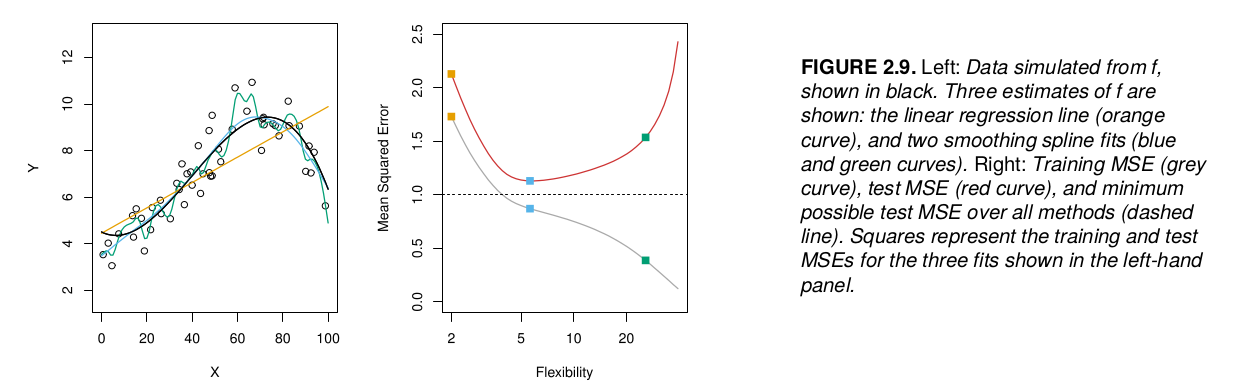
\includegraphics[width = 1\linewidth]{figures/03/figure_2_6.png}
\end{figure}
\begin{itemize}
\item True f is non-linear, orange linear fit is not flexible enough
\item Green curve (model with highest flexibility) has the lowest training MSE
\end{itemize}
As we know f we can compute test MSE as a function of flexibility.
\begin{itemize}
\item Test MSE is displayed using the \textbf{red} curve
\item As with the training MSE, the test MSE initially declines as the level of
flexibility increases.
\item Dashed line: irreducible error $Var(\epsilon)$, lowest achievable test MSE $\rightarrow$ Blue smoothing spline is close to optimal
\end{itemize}

\end{frame}

\begin{frame}
\frametitle{Overfitting - U-shaped Relationship of Flexibility and Test MSE}
Fundamental property of statistical learning
(independent of the data set):
\begin{itemize}
\item Training MSE decreases with increasing flexibility
\item Test MSE has U-shape
\end{itemize}
\bigskip
Overfitting the data:
\begin{itemize}
\item Small training MSE, large test MSE
\item We try too hard to find patterns in the data
\item We pick up random patterns (no properties of f)
\end{itemize}
\bigskip
Training MSE can in most cases be expected to
be smaller than test error
Overfitting is when a less flexible model would
have yielded smaller test MSE
\end{frame}

\begin{frame}
\frametitle{Example}
\begin{figure}
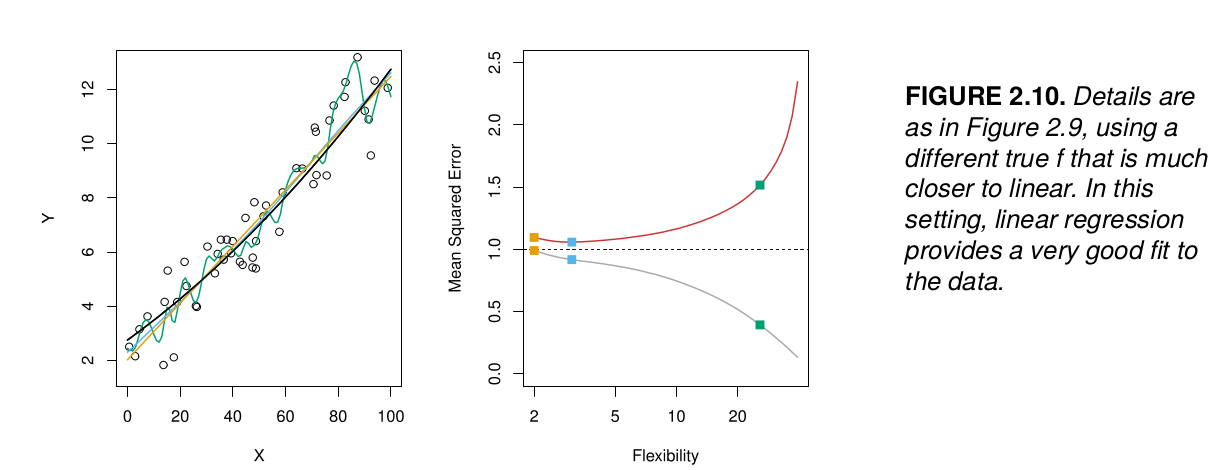
\includegraphics[width = 1\linewidth]{figures/03/figure_2_7.png}
\end{figure}
\end{frame}


\section{cross validation}
\begin{frame}
\frametitle{cross- validation motivation}
Why do we need cross validation?
\begin{itemize}
\item assess the predictive performance of the models and and to \textbf{ judge how they perform outside the sample to a new data set} also known as test data
\item The motivation to use cross validation techniques is that when we fit a model, we are fitting it to a training dataset.
\item  Without cross validation we only have information on how does our model perform to our in-sample data.
\item Ideally we would like to see how does the model perform when we have a new data in terms of accuracy of its predictions. In science, theories are judged by its predictive performance.
\end{itemize}

   
\end{frame}

\begin{frame}
\frametitle{k-fold cross validation}
Cross validation is sometimes also called rotation estimation:
\begin{figure}
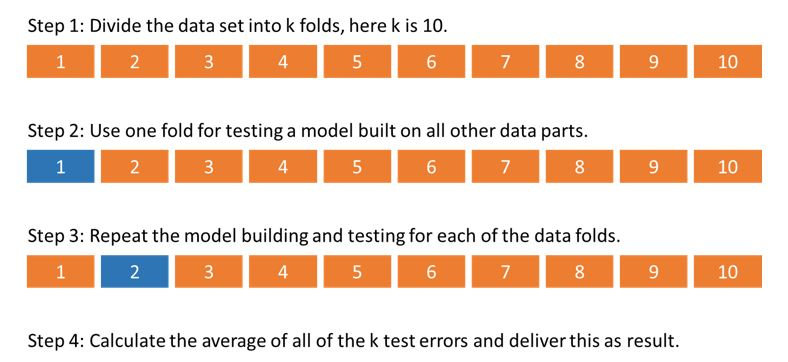
\includegraphics[width = 1\linewidth]{figures/03/blog3-2.jpg}
\end{figure}
With the k-fold cross validation we have a very clear estimate of the error when doing prediction.
\end{frame}

\begin{frame}
\frametitle{leave one out cross validation}
Leave one out cross validation is a special case of k-fold cross validation when $k \rightarrow n$:
\begin{figure}
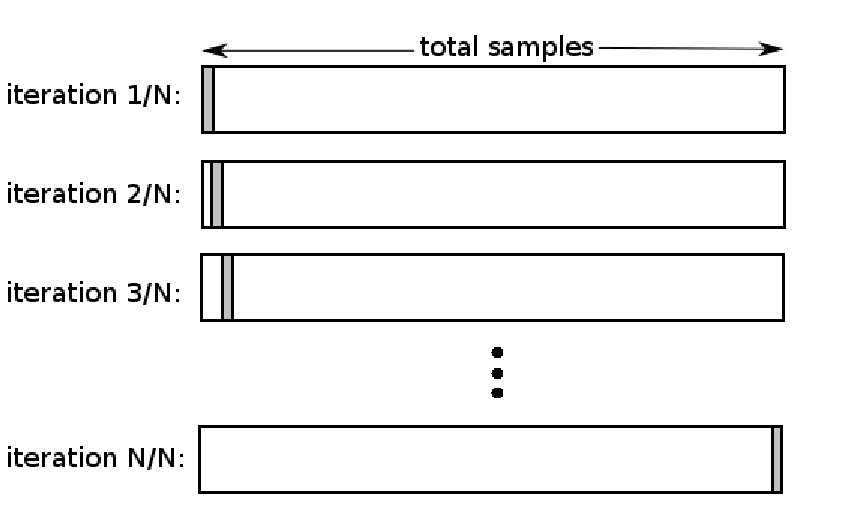
\includegraphics[width = 0.7\linewidth]{figures/03/Leave-One-Out-Cross-Validation.png}
\end{figure}
Now we train on all data but one observation and test on the one observation left out.
\end{frame}


\section{error metrics}
\subsection{regression}
\begin{frame}
\frametitle{Regression error metrics}
In the previous section we learned about the technique of evaluating machine learning models. Since we need to characterize a good or bad machine learning models we need the help of evaluation metrics:
\newline
\newline
In \textbf{regression} we want our model estimates $\hat{y}$ near the true points $y$. For this purpose we can calculate several distance metrics:
\newline
\begin{itemize}
\item Mean squared error (MSE): $\frac{1}{n} \sum_{i=1}^n (y_i - \hat{y_i})^2$
\item Root mean squared error (RMSE): $\sqrt[]{\frac{1}{n} \sum_{i=1}^n (y_i - \hat{y_i})^2} $
\item Mean absolute error (MAE): $\frac{1}{n} \sum_{i=1}^n |y_i - \hat{y_i}|$
\end{itemize}

\end{frame}

\subsection{classification}
\begin{frame}
\frametitle{Classification error metrics}
\textbf{Classification models assign a (discrete) class label} to an observations (in contrast to regression which assigns a (floating) value). 
\newline
Example classification tasks:
\begin{itemize}
\item will the client default his credit (yes, no)?
\item which of the three medical conditions (a, b, c) does the person have?
\end{itemize}
\bigskip
For these type of problems we need other evaluation metrics:
\begin{itemize}
\item error rate
\item accuracy
\item confusion matrix
\item f-Score
\item ...
\end{itemize}
\end{frame}

\begin{frame}
\frametitle{Binary classification }
Assume a binary classification task: e.g. will the client default his credit (yes, no)?
\newline
The evaluation on the test set gives us the following matrix:
\begin{figure}
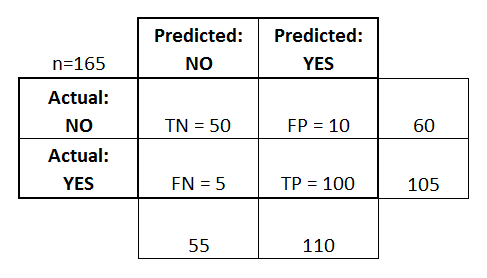
\includegraphics[width = 0.6\linewidth]{figures/03/confusion_matrix2.png}
%link: http://www.dataschool.io/content/images/2015/01/confusion_matrix2.png
\end{figure}
\end{frame}


\begin{frame}
\frametitle{classification - evaluation metrics}
\begin{figure}
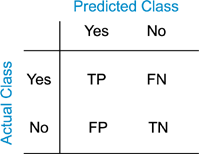
\includegraphics[width = 0.4\linewidth]{figures/03/Binary_confusion_matrix.png}
%link: https://upload.wikimedia.org/wikipedia/en/a/a6/Binary_confusion_matrix.png
\end{figure}
\begin{itemize}
\item accuracy: $\frac{TP + TN}{TP +FN +FP + TN}$
\item error rate: $\frac{FP + FN}{TP +FN +FP + TN} = 1- Accuracy$
\end{itemize}
\bigskip
\textbf{Question:} What is the accuracy \& error rate for the credit example? 
\end{frame}

\begin{frame}
\frametitle{F-Score (1) }
In many cases it is very useful to have a better understanding of the false classified samples.
\newline
Assume you want to predict breast cancer then you ideally want to weigh your false classified: 
\begin{itemize}
\item FN is high: you predict no breast cancer but there is actually one: person might die
\item FP is high: you predict breast cancer but there is actually none: high costs for medical procedure,...
\end{itemize}
\end{frame}

\begin{frame}
\frametitle{F-Score (2)}
\begin{itemize}
\item Precision ("Hit-Ratio"): $\frac{TP}{TP + FP}$
\item Recall (probability of detection): $\frac{TP}{TP + FN}$
\end{itemize}
We can aggregate Precision and Recall with the f-score
\newline
\begin{equation*}
F(\beta) = (1 + \beta^2) \frac{ precision * recall}{\beta^2 precision + recall}
\end{equation*}
often used $F(1)$-score:
\begin{equation*}
F(1) = 2* \frac{precision * recall}{precision + recall}
\end{equation*}
$F(1)$ is the harmonic mean of precision and recall. It is also called the traditional F-measure or balanced F-score.
\end{frame}


\begin{frame}
\Huge{\centerline{The End}}
\end{frame}

%----------------------------------------------------------------------------------------

\end{document}